\section{Experiments}
\label{sec:exp}

\paragraph{Protocol.}
Each repetition draws $n$ labelled and $N$ unlabelled records i.i.d.\ \emph{with replacement} from a pool of
the \texttt{ppi-python} 0.2.3 data (Table~\ref{tab:datasets}); the pool's empirical distribution is the population, so the truth is the pool
mean (for OLS, the pool fit), $Y$ is hidden on the unlabelled draw, and every method sees the same draw (paired comparisons).
Unless stated, $N=\min(\text{pool size},10^4)$ (the validity grid uses $2\times10^4$). Coverage is reported with Wilson 95\% intervals and widths as paired
ratios with confidence intervals; seeds, versions, commands and expected runtimes are in the reproduction notes.
Pools without a population truth or with a shift are used only as stated in the text where they appear.

\begin{table}[t]
\caption{Pools used for the mean. Skewness and $\mathrm{corr}(Y,\hat Y)$ are computed on the full pool; $\dim X$ is the number of
features available to the adjusters.}
\label{tab:datasets}
\centering
\small\begin{tabular}{lrlrrrr}
\toprule
pool & $N_{\mathrm{pool}}$ & outcome & mean $Y$ & skew $Y$ & corr$(Y,\hat Y)$ & $\dim X$ \\
\midrule
galaxies & 16{,}743 & binary & 0.259 & 1.1 & 0.74 & 0 \\
forest & 1{,}596 & binary & 0.152 & 1.9 & 0.54 & 0 \\
alphafold & 10{,}802 & binary & 0.177 & 1.7 & 0.82 & 0 \\
gene\_expression & 61{,}150 & continuous & 6.77 & 0.56 & 0.96 & 0 \\
census\_income & 380{,}091 & continuous & $4.31{\times}10^{4}$ & 4.7 & 0.61 & 2 \\
census\_healthcare & 318{,}215 & binary & 0.671 & $-$0.73 & 0.71 & 2 \\
census\_education & 318{,}215 & continuous & 17.8 & $-$1.8 & 0.63 & 4 \\
\bottomrule
\end{tabular}

\end{table}

\subsection{Validity of the baselines (C0)}
\label{sec:validity}
Width is only meaningful at valid coverage, so we first measure it. Figure~\ref{fig:validity} gives the coverage of nominal 95\%
intervals for classical, PPI and PPI++ (Wald, $t$, studentised bootstrap) on seven pools, 2000 repetitions per cell,
$n\in\{15,25,50,100,200,500\}$.
Wald PPI++ undercovers at small $n$ on skewed or rare-outcome pools: on \texttt{census\_income} its coverage is 0.755 at $n=15$,
0.907 at $n=200$ and 0.926 at $n=500$, and the Monte-Carlo standard error is about 0.5 percentage points at 2000 repetitions. The $t$ quantile
barely helps (0.787, 0.909, 0.928). The studentised bootstrap repairs most of this on \texttt{census\_income} (0.906, 0.929, 0.951) but
over-corrects at $n=15$ on the small, rare-outcome pools (\texttt{forest} 0.658, \texttt{alphafold} 0.698). On the other six pools the shortfall of PPI++ Wald is 1.1 to 7.9 percentage points at $n=50$ and 0 to 2.2 at $n=200$, and at $n=500$ it is
within 1 percentage point of nominal on all six (0.942 to 0.953); \texttt{gene\_expression} is the closest throughout (0.946 at $n=100$). The consequence for what follows is that the useful comparison of widths is \emph{like for like}: an adjuster
is compared with PPI++ calibrated in the same way, and no comparison against an undercovering interval is read as a saving.

\begin{figure}[t]
\centering
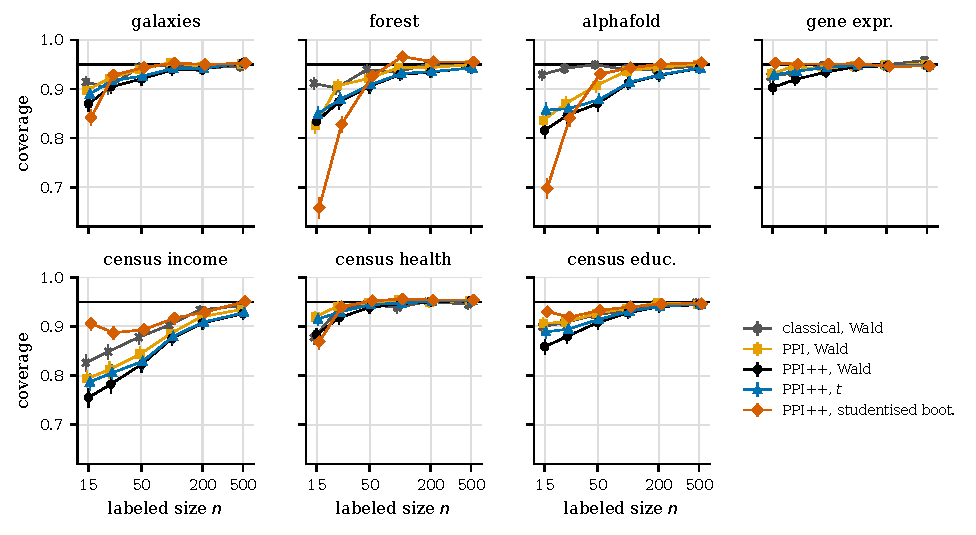
\includegraphics[width=\linewidth]{figures/fig_validity.pdf}
\caption{Coverage of 95\% intervals against labelled size $n$ on seven pools (2000 repetitions per cell; i.i.d.\ with replacement from the pool;
$N=\min(\text{pool},2\times10^4)$; truth = pool mean). Bars: Wilson 95\% intervals; line: nominal level.}
\label{fig:validity}
\end{figure}

\subsection{Population headroom of control variates built from $(f,X)$ (C1)}
\label{sec:headroom}
How much shorter can any adjuster be, if estimated well? Figure~\ref{fig:headroom} shows the asymptotic width ratio
to PPI++ (large $N$) of each adjuster class fitted on the whole pool with 2-fold cross-fitting, with the standard deviation over ten random splits.
On the seven pools the best ratio is 0.988 (\texttt{gene\_expression}, isotonic), 0.995 (\texttt{census\_income}, gradient boosting on $(f,X)$),
0.999 or above elsewhere: at most about 1.2\% in width for the classes tried (a lower bound on the true headroom, since the adjusters are fitted on half-pools), and the best ratio lies inside the grey band of $\pm1\%$ for six of the seven pools. PPI with $\lambda=1$ is
wider than PPI++ on \texttt{gene\_expression} (ratio 1.106) and \texttt{census\_income} (1.022), where $f$ is on a different scale from $Y$; classical
intervals are 1.19 to 3.73 times wider than PPI++. Ratios above one for flexible classes (e.g.\ boosting on \texttt{forest}, 1.021) reflect
the estimation error of an adjuster fitted on half of a 1596-record pool, not a loss of the bound. For the mean on these pools PPI++ is therefore
within about one percent of what any adjuster of the classes tried could reach; whether even that is attainable at the sizes of a labelled set is the
question of the following sections.

\begin{figure}[t]
\centering
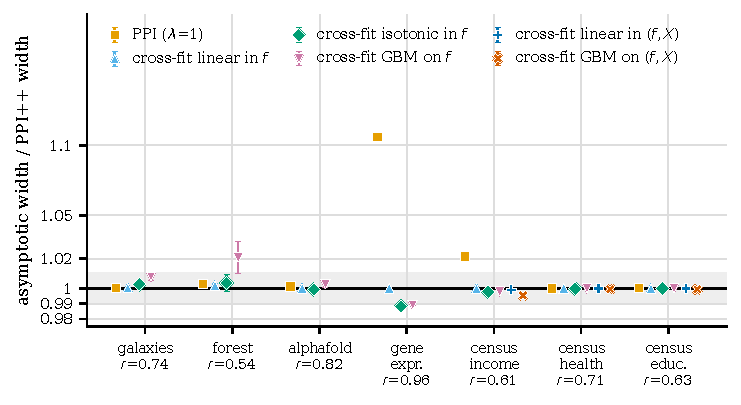
\includegraphics[width=\linewidth]{figures/fig_headroom_population.pdf}
\caption{Population headroom: asymptotic CI-width ratio of the best control variate in each class to power-tuned PPI++ (1 = parity, $<1$ narrower).
Each class is fitted by 2-fold cross-fitting on the full pool; error bars are the standard deviation over ten random splits (split noise only).
Grey band: $\pm1\%$. $r=\mathrm{corr}(Y,f)$.}
\label{fig:headroom}
\end{figure}
